\pagebreak
\section{Setting up end devices}
Unikernels, similar to traditional operating systems can be booted directly from BIOS to hardware. Nevertheless, this is not flexible enough for cloud computing standards, so hypervisors are used for on demand provisioning of unikernels. For proof of concept development, many different end device configurations were used. There are two different usage scenarios in mind when configuring devices. First one is hypervisor-enabled unikernel runtime and the other one is with IoT.

For hypervisor-enabled runtime, a laptop was used. Installing a hypervisor on conventional virtual machines in the cloud was not possible because it breaks internal networking and makes it impossible to access machines from outside. Although it might be possible for some cloud providers, it's not a good testing environment as accessing to BIOS of a cloud provided virtual machine is not possible.

The mentioned laptop has Debian as the host operating system and Xen was installed through Debian with administrative privileges to access BIOS. After Xen is installed, when laptop is booted up, user can select to start Debian with Xen enabled or not. It's the same interface that a user sees when dual boots e.g. Windows with Linux. Starting with the Xen option gives xen daemon access to manipulate hardware. Because a linux system is installed on the computer that communicates with the hypervisor, it's a straightforward process to write Kubernetes clients. That laptop is connected to Kubernetes cluster through a valid kubeconfig file. Figure \ref{fig:hypervisor} shows the final overview of the setup. The virtual-kubelet runs on Debian and communicates with Xen trough xen-cli, \textbf{xl}. Two additional Linux VMs are traditional Kubernetes nodes connected with kubelet and they are running on the LRZ cloud.

\begin{figure}[htpb]
  
  \centering
  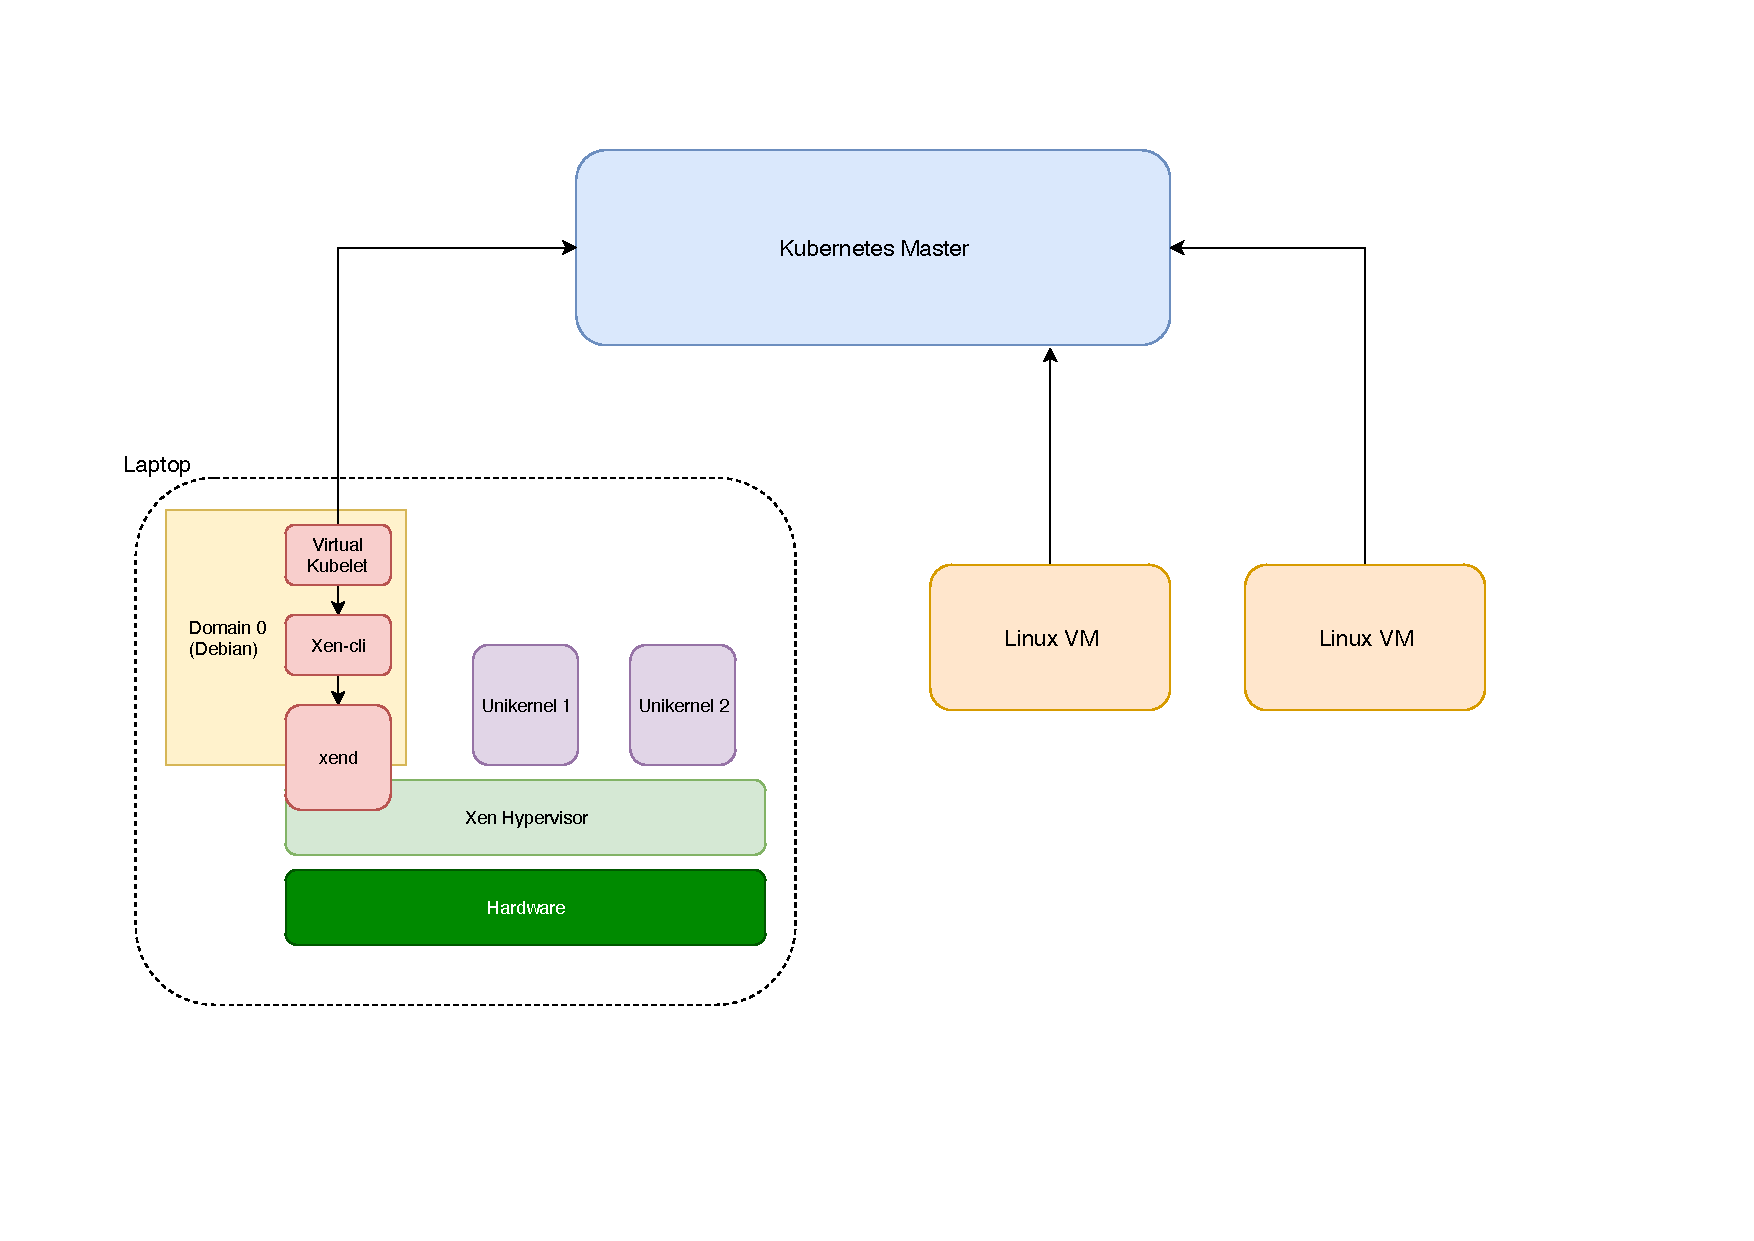
\includegraphics[width=1.2\textwidth]{figures/arch_new.pdf}
  \caption{ Kubernetes cluster with a single hypervisor-enabled node for unikernel deployment} \label{fig:hypervisor}
\end{figure}


For further testing, a VM with Docker runtime was created. This VM does not have a kubelet and runs only virtual-kubelet to communicate with the Kubernetes cluster. It still runs Docker containers. The provider for that case was called \textit{Docker}. It was just for exercising the virtual-kubelet API and is not part of the final setup.

To experiment more with the unikernel ecosystem, Solo5 \cite{solo5} was installed alongside Xen to the aforementioned laptop. Solo5 can be built on top of Qemu or KVM and it markets itself as a unikernel specific runtime. To test Solo5, Qemu was installed because the hardware didn't allow KVM virtualisation.

Another enviroment is Docker containers running virtual-kubelet. They are built on top Ubuntu base image and unikernels can run on them. They are being used to simulate hundreds of IoT machines, since both Docker and Raspberry Pi lack hypervisor technology.

When configuring end devices for hypervisors, a network interface for unikernels should be set. If a unikernel application is using networking, the network interface of the host should be given to the boot up command to make it get an IP from local DHCP.


For IoT devices, Raspberry Pi 3 was used. Raspberry Pi uses ARM processor and AMD64 hypervisors can't be ported easily to ARM. There is also not too much motivation for it, because Raspberry Pi is not a powerful end-device and not many virtualisation can be done on it. Despite that, there are projects for lightweight virtualisation on Raspberry Pi. For more powerful end-devices though, there are hypervisor projects but they are out of scope for this thesis.

Despite lack of virtualisation, it's possible to run unikernels on Raspberry Pi by selecting Unix as the compilation target. Virtual-kubelet can also be compiled to ARM architecture and only takes 31 MB. A test setup was created with the circuit in \ref{fig:rpi-diagram}.

\begin{figure}[htpb]
  \centering
  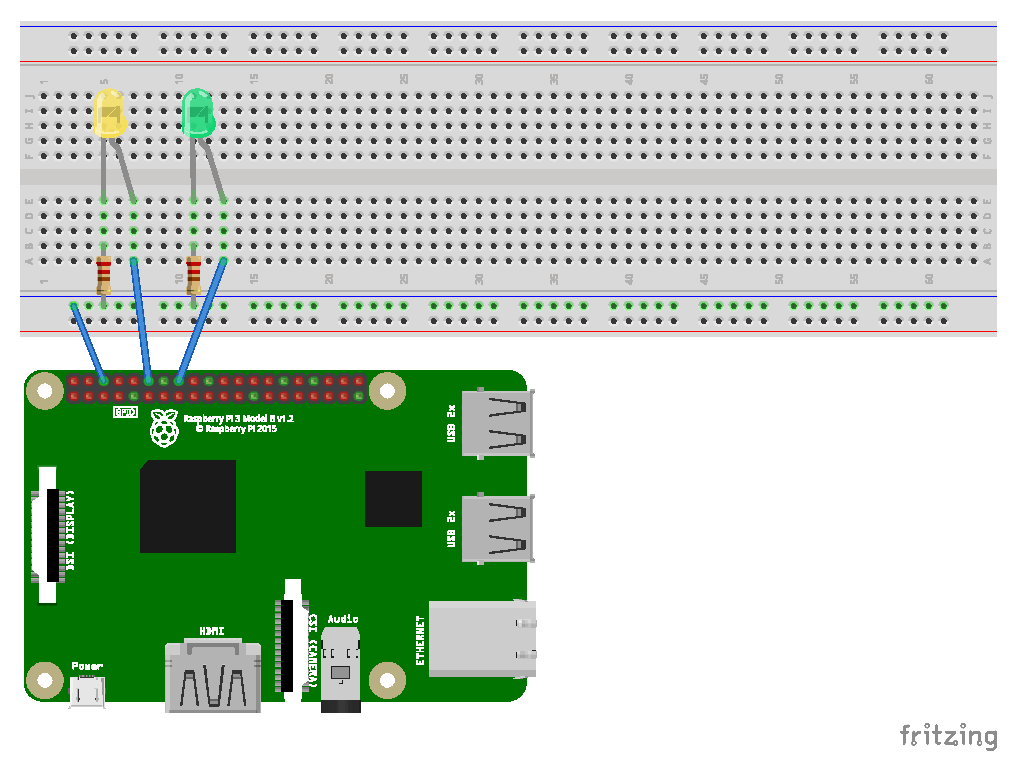
\includegraphics[height=0.6\textwidth]{figures/rpi-diagram.pdf}
  \caption{Yellow connected to pin 18 and green to pin 23} \label{fig:rpi-diagram}
\end{figure}

For the IoT case, two different DaemonSets are deployed to the cluster, namely yellow-daemon and green-daemon. Both DaemonSets are configured to deploy to nodes labeled with \textit{model=raspberry-pi}. While yellow-daemon is deployed to every node, green-daemon is only deployed to nodes if they have the \textit{light=GREEN} label additional to the raspberry-pi label. When a new device connects to cluster through virtual-kubelet, yellow-daemon deploys a unikernel application that turns the yellow led on. This workflow simulates the auto-configuration ability of this solution. The logic of the deployed application can be replaced with e.g. downloading additional binaries, sending GPS data only once, setting up a local network, etc.


When Raspberry Pi is labeled with \textit{light=GREEN}, green-daemon deploys a unikernel that toggles the green light every 2 second. When the label is removed, virtual-kubelet kills the unikernel, which returns the green led to OFF state upon graceful termination. The unikernel applications get the pin number as a command-line argument. If a change occurs on the pin number that the led is connected to, the daemon can be edited on the fly with \textit{kubectl edit daemonset green-daemon} and the new pin number can be given to the \textbf{args} field. Termination of the unikernel with the outdated pi number and creation of the new one is handled completely by the Kubernetes API. The full YAML file for the mentioned DaemonSet can be seen in \ref{fig:green-daemon}.



